\documentclass{beamer}
\usetheme{Boadilla}
\usecolortheme{sidebartab}
\beamertemplatenavigationsymbolsempty
\setbeamertemplate{footline}[frame number]
\usepackage{hyperref} 
\usepackage{graphicx}
\usepackage{color}
\usepackage{booktabs}
\usepackage{listings}
\usepackage{soul}
\usepackage{tikz}
\usepackage[utf8]{inputenc}
\usepackage{CJKutf8}
\usetikzlibrary{shapes.geometric}

\definecolor{gray}{rgb}{0.4,0.4,0.4}
\definecolor{darkblue}{rgb}{0.0,0.0,0.6}
\definecolor{cyan}{rgb}{0.0,0.6,0.6}

\lstset{
	basicstyle=\ttfamily,
	columns=fullflexible,
	showstringspaces=false,
	commentstyle=\color{gray}\upshape
}

\tikzset{node style/.style={
		draw=blue,
		thick,
		fill=blue!70,
		text=white,
		ellipse,
		minimum width=2cm,
		minimum height=0.75cm,
		font=\small,
		outer sep=3pt,
	},
	blank style/.style={
		draw=black,
		thick,
		fill=white,
		text=white,
		ellipse,
		minimum width=2cm,
		minimum height=0.75cm,
		font=\small,
		outer sep=3pt,
	},
	literal style/.style={
		draw=red,
		thick,
		fill=red!70,
		text=white,
		rectangle,
		minimum width=2cm,
		minimum height=0.75cm,
		font=\small,
		outer sep=3pt,
	},
	edge style/.style={
		#1,
		text=black,
		font=\footnotesize,
		above
	}
}

\makeatletter
\newcommand\SoulColor{%
	\let\set@color\beamerorig@set@color
	\let\reset@color\beamerorig@reset@color}
\makeatother

\lstset{language=XML}

\title{SPARQL: Fortgeschrittene Themen}
\author{Markus Stocker}
\date{28. Mai 2018}

\begin{document}

\maketitle

\begin{frame}{Rekapitulation}
	
	\begin{itemize}
		\item Was ist SPARQL und warum benötigt man sowas?
		\item Was ist ein \emph{triple pattern}? Wie unterscheidet es sich von einem \emph{triple}?
		\item Wozu dienen Variablen in SPARQL?
		\item Was ist ein \emph{basic graph pattern}?
		\item Womit kann man Resultatsmengen einschränken?
	\end{itemize}
	
\end{frame}

\begin{frame}[fragile]{Rekapitulation: Erklären Sie diese Abfrage}
	
	\small
	\begin{lstlisting}
  PREFIX ex: <http://example.org#> 
  PREFIX rdf: <http://www.w3.org/1999/02/22-rdf-syntax-ns#>
  PREFIX rdfs: <http://www.w3.org/2000/01/rdf-schema#>
	
  SELECT ?label ?radius
  WHERE {
    ?planet rdf:type ex:Planet .
    ?planet rdfs:label ?label .
    OPTIONAL { 
       ?planet ex:radius ?radius 
       FILTER (?radius > 6000)
    }
  }
	\end{lstlisting}
	
\end{frame}

\begin{frame}{Übersicht}
	
	\begin{itemize}
		\item Resultatformate
		\item Modifizierer
		\item SPARQL Update
		\item SPARQL Endpoints
		\item Abfragenoptimierung
	\end{itemize}
	
\end{frame}

\begin{frame}{Resultatformate}
	
	\begin{itemize}
		\item \texttt{SELECT}: Variabeln und deren Ersetzungen
		\item \texttt{CONSTRUCT}: RDF Dokument
		\item \texttt{ASK}: Wahr oder falsch
		\item \texttt{DESCRIBE}: RDF Ressourcen beschreiben
	\end{itemize}
	
\end{frame}

\begin{frame}{Resultatformate: \texttt{SELECT}}
	
	\begin{itemize}
		\item Das \texttt{SELECT} Format haben wir bereits gesehen
		\item Angabe einer oder mehrerer Variabeln
		\item Oder \texttt{*} als Kurzform für alle Variabeln die in der Abfrage vorkommen
		\item Die Variabelnersetzungen (Resultate) werden als Tabelle angezeigt
		\item Die Tabellendarstellung hat auch Nachteile
		\item Zum Beispiel, nicht unbedingt geeignet für Weiterverarbeitung
		\item Aber auch ungewünschte Redundanz (Werte in einer Spalte)
	\end{itemize}
	
\end{frame}


\begin{frame}{Resultatformate: \texttt{CONSTRUCT}}
	
	\begin{itemize}
		\item Resultate werden als RDF Dokument zurückgegeben
		\item \texttt{CONSTRUCT} erwartet ein \emph{template} für das zurückgegebene RDF
		\item Ein \emph{template} kann flexibel gestaltet werden
		\item Neue Tripel oder spezifische Werte einführen, Prädikate ersetzen
		\item Das resultierende RDF kann direkt weiterverarbeitet werden
	\end{itemize}
	
\end{frame}

\begin{frame}[fragile]{\texttt{CONSTRUCT}: Beispiel}
	
	\small
	\begin{lstlisting}
  PREFIX ex: <http://example.org#> 
  PREFIX rdf: <http://www.w3.org/1999/02/22-rdf-syntax-ns#>
  PREFIX rdfs: <http://www.w3.org/2000/01/rdf-schema#>
	
  CONSTRUCT {
    ?planet rdf:type ex:Planet .
    ?planet rdf:type ex:TerrestrialPlanet .
    ?planet rdfs:label ?label .
    ?planet ex:radius ?radius .
  }
  WHERE {
    ?planet rdf:type ex:Planet .
    ?planet rdfs:label ?label .
    ?planet ex:radius ?radius .
    FILTER (?radius > 2000 & ?radius < 8000)
  }
	\end{lstlisting}
	
\end{frame}

\begin{frame}{Resultatformate: \texttt{ASK}}
	
	\begin{itemize}
		\item Resultat ist entweder \emph{true} oder \emph{false}
		\item \emph{True} wenn die Abfrage zutreffende Resultate liefert, sonst \emph{false}
		\item Kann benutzt werden um zu testen ob es Resultate gibt
	\end{itemize}
	
\end{frame}

\begin{frame}[fragile]{\texttt{ASK}: Beispiel}
	
	\small
	\begin{lstlisting}
  PREFIX ex: <http://example.org#> 
  PREFIX rdf: <http://www.w3.org/1999/02/22-rdf-syntax-ns#>
	
  ASK {
    ?planet rdf:type ex:Planet .
  }
	\end{lstlisting}
	
\end{frame}

\begin{frame}{Resultatformate: \texttt{DESCRIBE}}
	
	\begin{itemize}
		\item Damit kann man RDF navigieren ohne die Struktur zu kennen
		\item Die einfachste \texttt{DESCRIBE} Abfrage ist für eine einzelne Ressource
		\item \texttt{DESCRIBE <http://example.org\#Earth>} 
		\item Variabelersetzte Ressourcen können auch beschrieben werden
	\end{itemize}
	
\end{frame}

\begin{frame}[fragile]{\texttt{DESCRIBE}: Beispiel}
	
	\small
	\begin{lstlisting}
  PREFIX ex: <http://example.org#> 
  PREFIX rdf: <http://www.w3.org/1999/02/22-rdf-syntax-ns#>
	
  DESCRIBE ?planet 
  WHERE {
    ?planet rdf:type ex:Planet .
    ?planet ex:radius ?radius .
    FILTER (?radius > 6000)
  }
	\end{lstlisting}
	
\end{frame}

\begin{frame}{Modifizierer}
	
	\begin{itemize}
		\item Oft ist nicht bekannt wie gross eine Resultatsmenge sein wird
		\item Oft ist die Menge viel zu gross und für Benutzer nicht brauchbar
		\item Abhilfe bieten Operatoren die die Ergebnissequenz steuern und ändern
		\item Zum Beispiel, Sortierung steuern und Ergebnismenge limitieren
		\item Man kann so z.B. die \emph{top 10} Resultate erhalten
	\end{itemize}
	
\end{frame}

\begin{frame}[fragile]{Modifizierer: \texttt{ORDER BY}}
	
	\begin{itemize}
		\item Sortierung in auf- (\texttt{ASC}) oder absteigender (\texttt{DESC}) Reihenfolge
		\item Sinnvol nur im Zusammenhang mit \texttt{SELECT} Abfragen
	\end{itemize}
	
	\small
	\begin{lstlisting}
  PREFIX ex: <http://example.org#> 
  PREFIX rdf: <http://www.w3.org/1999/02/22-rdf-syntax-ns#>
  PREFIX rdfs: <http://www.w3.org/2000/01/rdf-schema#>
	
  SELECT ?label ?radius
  WHERE {
    ?planet rdf:type ex:Planet .
    ?planet rdfs:label ?label .
    ?planet ex:radius ?radius .
  }
  ORDER BY DESC(?radius)
	\end{lstlisting}
	
\end{frame}

\begin{frame}[fragile]{Modifizierer: \texttt{LIMIT} und \texttt{OFFSET}}
	
	\begin{itemize}
		\item Ermöglicht die Adressierung eines Ausschnitts der Resultatsmenge
		\item Stückweise Verarbeitung der Resultatsmenge
		\item Folgendes Beispiel sind die \emph{top 10} Resultate
	\end{itemize}
	
	\small
	\begin{lstlisting}
  PREFIX ex: <http://example.org#> 
  PREFIX rdf: <http://www.w3.org/1999/02/22-rdf-syntax-ns#>
  PREFIX rdfs: <http://www.w3.org/2000/01/rdf-schema#>
	
  SELECT ?label ?radius
  WHERE {
    ?planet rdf:type ex:Planet .
    ?planet rdfs:label ?label .
    ?planet ex:radius ?radius .
  }
  ORDER BY DESC(?radius) LIMIT 10 OFFSET 0
	\end{lstlisting}
	
\end{frame}

\begin{frame}{SPARQL Update}
	
	\begin{itemize}
		\item Bis anhin haben wir nur Abfragen gestellt
		\item Also, deklarativer Zugriff auf Information in RDF
		\item Man kann Information in RDF mittels SPARQL auch ändern
		\item Insbesondere neue Information hinzufügen oder löschen
		\item Wurde mit SPARQL 1.1 eingeführt
	\end{itemize}
	
\end{frame}

\begin{frame}[fragile]{SPARQL Update: \texttt{INSERT (DELETE) DATA}}
	
	\small
	\begin{lstlisting}
  PREFIX ex: <http://example.org#> 
  PREFIX rdf: <http://www.w3.org/1999/02/22-rdf-syntax-ns#>
  PREFIX rdfs: <http://www.w3.org/2000/01/rdf-schema#>
	
  INSERT DATA
  {
	ex:Mars rdf:type ex:Planet .
	ex:Mars rdfs:label "Mars" .
  }
	\end{lstlisting}
	
\end{frame}

\begin{frame}[fragile]{SPARQL Update: \texttt{DELETE/INSERT}}
	
	\small
	\begin{lstlisting}
  PREFIX ex: <http://example.org#> 
  PREFIX rdf: <http://www.w3.org/1999/02/22-rdf-syntax-ns#>
  PREFIX rdfs: <http://www.w3.org/2000/01/rdf-schema#>
	
  DELETE { ?planet rdf:type ex:Planet }
  INSERT { ?planet rdf:type ex:TerrestrialPlanet } 
  WHERE {
    ?planet rdf:type ex:Planet .
    ?planet ex:radius ?radius .
    FILTER (?radius > 2000 & ?radius < 8000)
  }
	\end{lstlisting}
	
\end{frame}


\begin{frame}{SPARQL Endpoints}
	
	\begin{itemize}
		\item Web Service für SPARQL Abfragen auf RDF Datenbank
		\item Üblicherweise mit graphischer und Programmierschnittstelle
		\item Endpoints implementieren SPARQL Protokoll
		\item Das Übermittlungsprotokoll für Abfragen und Resultate
		\item Übermittlung von Resultaten auch in verschiedene Formate
		\item Zum Beispiel XML oder CSV
	\end{itemize}
	
\end{frame}

\begin{frame}[fragile]{SPARQL Endpoints: Beispiel DBpedia}
	
	\begin{itemize}
		\item Gehen Sie mal auf \texttt{http://dbpedia.org/sparql/}
		\item Und kopieren Sie die folgende Abfrage ins Textfeld
		\item Führen Sie die Abfrage dann aus (\emph{Run Query})
	\end{itemize}
	
	\small
	\begin{lstlisting}
  PREFIX dbo: <http://dbpedia.org/ontology/>
  PREFIX rdfs: <http://www.w3.org/2000/01/rdf-schema#>

  SELECT ?populationMetro ?populationTotal ?federalState ?country
  WHERE {
    [] rdfs:label "Hannover"@de ;
       dbo:populationMetro ?populationMetro ;
       dbo:populationTotal ?populationTotal ;
       dbo:federalState ?federalState ;
       dbo:country ?country
  }
	\end{lstlisting}
	
\end{frame}

\begin{frame}{Etwas aus der Eigenen Küche: Abfragenoptimierung}
	
	\centering
	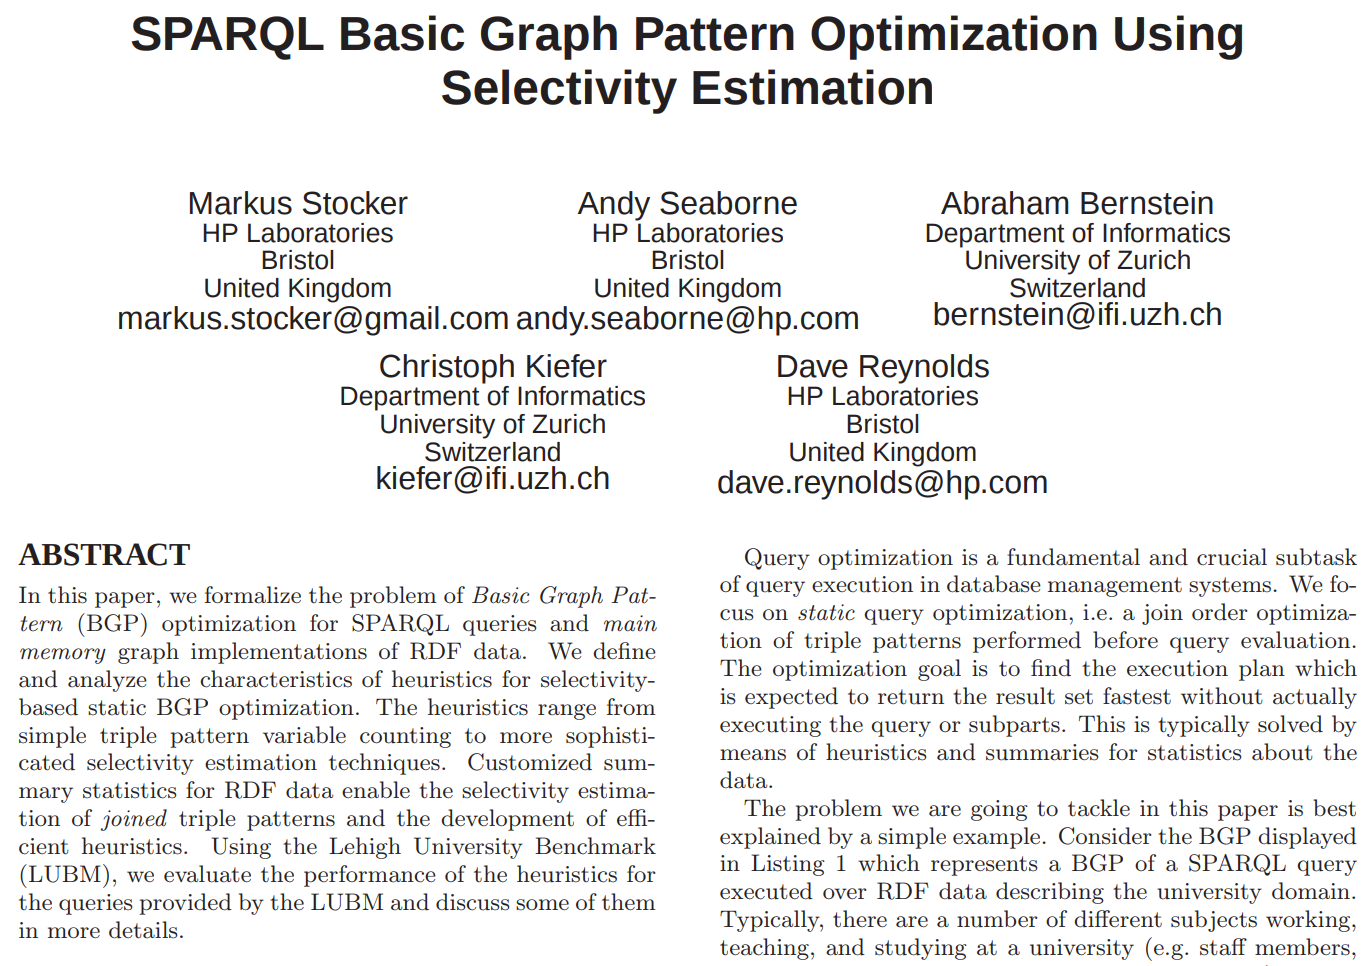
\includegraphics[scale=0.8]{optimization.png}
	
	\vspace{0.2cm}\scriptsize
	https://doi.org/10.1145/1367497.1367578
	
\end{frame}

\begin{frame}{Abfragenoptimierung}
	
	\begin{itemize}
		\item Die \emph{triple patterns} werden der Reihe nach ausgeführt (naiv)
		\item Jedes ergibt eine Menge als Zwischenresultat
		\item Zudem gibt es auch \emph{joins} zwischen \emph{triple patterns}
		\item Daraus können sich sehr grosse Zwischenresultate ergeben
		\item Es macht Sinn, die selektivsten \emph{triple patterns} zuerst auszuführen
		\item Sprich die die möglichst kleine Zwischenresultatsmengen ergeben
		\item So kann man die Abfrage optimieren
		\item Also die Abfragegeschwindigkeit potentiell drammatisch verbessern
		\item Die meisten Systeme implementieren heute solche Optimierungen
	\end{itemize}
	
\end{frame}

\begin{frame}{Zusammenfassung}
	
	\begin{itemize}
		\item Zusätzlich zu \texttt{SELECT} gibt es auch \texttt{CONSTRUCT}
		\item Und \texttt{ASK} und \texttt{DESCRIBE} Abfragen
		\item Resultatsmengen können geordnet und limitiert werden
		\item SPARQL Update ist eine wichtige Erweiterung
		\item SPARQL Endpoints als verteilte RDF Datenbanken
	\end{itemize}
	
\end{frame}

\end{document}